% Begin the document and set up the style of the document
\documentclass[a4paper]{article}

% Install the required packages for the document 
\usepackage{envmath}
\usepackage{esvect}
\usepackage{graphicx}
\usepackage{gensymb}
\usepackage{tikz}
\usepackage[mathcal]{euscript}
\usepackage{geometry}
\usepackage{enumitem}
\usepackage{mathtools}
\usepackage{graphicx}
\usepackage{amsmath}
\usepackage{amscd}
\usepackage{amssymb}
\usepackage{amsfonts}
\usepackage{harpoon}
\usepackage{pgf}
\usepackage{tikz}
\usepackage{mathrsfs}
\usepackage{asyalign}
\usepackage{physics}
\usepackage{enumitem}
\usepackage{xhfill}
\usepackage{accents}
\usepackage{cite}
\usepackage{url}
\usepackage[tableposition=top]{caption}
\usepackage{ifthen}
\usepackage[utf8]{inputenc}
\usepackage{tikz-3dplot}
\usetikzlibrary{patterns}
\usetikzlibrary{arrows}

\DeclareMathOperator\cis{cis}
\DeclareMathOperator\Arg{Arg}

% Page and style settings
\parskip=8pt
\parindent=0pt
% Right margin
\textwidth=6.25in
% Left margin
\oddsidemargin=0pt
\evensidemargin=0pt
% Bottom margin
\textheight=10in
% Top margin
\topmargin=-0.75in
\baselineskip=11pt
% end of page and other style settings

\renewcommand{\familydefault}{\sfdefault}


% Begin the text of the document
\begin{document}

% Begin the Title Page
\begin{titlepage}

\newcommand{\HRule}{\rule{\linewidth}{0.5mm}} % Defines a new command for the horizontal lines, change thickness here

\center % Center everything on the page
 
\textsc{\LARGE University of Sydney}\\[1.5cm] % Name of your university/college
\textsc{\Large MATH 1907}\\[0.5cm] % Major heading such as course name
\textsc{\large SSP}\\[0.5cm] % Minor heading such as course title

\HRule \\[0.4cm]
{ \huge \bfseries Assignment 1 - Fluid Dynamics and Conformal Transformations}\\[0.4cm] % Title of your document
\HRule \\[1.5cm]

\begin{minipage}{0.4\textwidth}
\begin{flushleft} \large
\emph{Author:}
Keegan Gyoery % Your name
\\
\emph{SID:}
470413467
\end{flushleft}
\end{minipage}
~
\begin{minipage}{0.4\textwidth}
\begin{flushright} \large
\emph{Lecturer:} 
Sharon Stephen % Tutor's Name
\\
\emph{Seminar:}
New Law Annexe SR 346
Tuesday 4pm
\end{flushright}
\end{minipage}\\[4cm]

{\large \today}\\[3cm] % Date, change the \today to a set date if you want to be precise

\vfill % Fill the rest of the page with whitespace

\end{titlepage}

\pagenumbering{arabic}
%%%%%%%%%%%%%%%%%%%%%%%%%%%
%%%%%%%%%%%%%%%%%%%%%%%%%%%
%%%%%%%%%%%%%%%%%%%%%%%%%%%
%%%%%%%%%%%%%%%%%%%%%%%%%%%

\begin{enumerate}[label=\textbf{\arabic*.}]

	\item Consider the two-dimensional, steady, incompressible, inviscid, irrotational fluid past the semi-circular cyclinder of radius 1 shown below.

	\begin{center}
	\begin{tikzpicture}
		% X - axis
		\draw[->] (-5,0)--(5,0) node[right]{$x$};
		% Y - axis
		\draw[->] (0,0)--(0,4) node[above]{$y$};
	  	% Circle
	  	\draw[very thick] (2,0) arc (0:180:2);

	  	\draw[very thick] (2,0)--(5,0);

	  	\draw[very thick] (-2,0)--(-5,0);

	  	\node at (-2,-0.3){$-1$};

	  	\node at (2,-0.3){$1$};

	  	\draw[->] (-5,3)--(-4,3);
	  	\draw[->] (-5,2.5)--(-4,2.5);
	  	\draw[->] (-5,2)--(-4,2);

	  	\node at (-5.25,2.5){$U$};

	\end{tikzpicture}
	\end{center}

	\begin{enumerate}

		\item 
		\begin{enumerate}

			\item By definition, an analytic function is conformal at any point if the derivative of the function is non-zero, and defined at that point. Using this definition, we will now show that the transformation $\displaystyle{\zeta = f(z) = z + \frac{1}{z}}$ is conformal at all points except $\displaystyle{z=0}$ and $\displaystyle{z=\pm 1}$.

			\begin{align*}
			\zeta & = z + \frac{1}{z}\\
			\therefore \frac{d\zeta}{dz} & = 1 + \frac{-1}{z^2}\\
			& = 1 - \frac{1}{z^2}\dots\dots\dots\dots(*)\\
			& = \frac{1}{z^2}\left(z^2-1\right)\\
			& = \frac{1}{z^2}\left(z-1\right)\left(z+1\right)\\
			\therefore \frac{d\zeta}{dz} & = 0 \hspace{5mm} \text{when $\displaystyle{z=\pm 1}$}\\
			\end{align*}

			Therefore $\displaystyle{\zeta = z + \frac{1}{z}}$ is not conformal when $\displaystyle{z=\pm 1}$, and when $\displaystyle{z=0}$, as it is undefined at $\displaystyle{z=0}$.

			\bigbreak

			\item We are now required to prove that the transformation $\displaystyle{\zeta = \xi + i\eta = z + \frac{1}{z}}$ maps the boundary of the domain shown above to the $\displaystyle{\xi}$ axis in the $\displaystyle{\zeta}$-plane and the region above the boundary to the upper-half of the $\displaystyle{\zeta}$-plane. In order to prove this result, we define $\displaystyle{z\coloneqq re^{i\theta}}$. Thus the following proofs will give us the required result.

			\bigbreak

			Firstly, we shall consider the semi-cicrular section of the function, with $\displaystyle{r=1}$, and $\displaystyle{\theta \in [0,\pi]}$. Thus the result of mapping $\displaystyle{z}$ to $\displaystyle{\zeta}$ is as follows.

			\begin{align*}
			\zeta & = z + \frac{1}{z}\\
			& = e^{i\theta} + \frac{1}{e^{i\theta}}\\
			& = e^{i\theta} + e^{-i\theta}\\
			& = \cos\theta + i\sin\theta + \cos\theta - i\sin\theta\\
			& = 2\cos\theta\\
			\therefore \xi + i\eta & = 2\cos\theta\\
			\therefore \xi & = 2\cos\theta\\
			\therefore \eta & = 0\\
			\end{align*}

			Thus the conformal transformation maps the semi-circular region to the $\displaystyle{\xi}$ axis for $\displaystyle{\xi \in [-2,2]}$, as $\displaystyle{\eta = 0}$, and $\displaystyle{2\cos\theta \in [-2,2]}$. 

			\pagebreak

			Now we shall consider the section of the function with $\displaystyle{r \in (-\infty,-1]}$, and $\displaystyle{\theta = \pi}$. Thus the result of mapping $\displaystyle{z}$ to $\displaystyle{\zeta}$ is as follows.

			\begin{align*}
			\zeta & = z + \frac{1}{z}\\
			& = re^{i\pi} + \frac{1}{re^{i\pi}}\\
			& = re^{i\pi} + \frac{1}{r}e^{-i\pi}\\
			& = r(-1) + \frac{1}{r}(-1)\\
			& = -r - \frac{1}{r}\\
			\therefore \xi + i\eta & = -\left(r + \frac{1}{r}\right)\\
			\therefore \xi & = -\left(r + \frac{1}{r}\right)\\
			\therefore \eta & = 0\\
			\end{align*}

			The range of $\displaystyle{\xi = -\left(r + \frac{1}{r}\right)}$ is $\displaystyle{\xi \in (-\infty,-2]}$, and thus the line segment specified above from the $\displaystyle{x}$ axis maps to the $\displaystyle{\xi}$ axis for $\displaystyle{\xi \in (-\infty,-2]}$.

			\bigbreak

			Now we shall consider the section of the function with $\displaystyle{r \in [1,\infty)}$, and $\displaystyle{\theta = 0}$. Thus the result of mapping $\displaystyle{z}$ to $\displaystyle{\zeta}$ is as follows.

			\begin{align*}
			\zeta & = z + \frac{1}{z}\\
			& = re^{i(0)} + \frac{1}{re^{i(0)}}\\
			& = re^{i(0)} + \frac{1}{r}e^{-i(0)}\\
			& = r(1) + \frac{1}{r}(1)\\
			& = r + \frac{1}{r}\\
			\therefore \xi + i\eta & = r + \frac{1}{r}\\
			\therefore \xi & = r + \frac{1}{r}\\
			\therefore \eta & = 0\\
			\end{align*}

			The range of $\displaystyle{\xi = \left(r + \frac{1}{r}\right)}$ is $\displaystyle{\xi \in [2,\infty)}$, and thus the line segment specified above from the $\displaystyle{x}$ axis maps to the $\displaystyle{\xi}$ axis for $\displaystyle{\xi \in [2,\infty)}$.

			\bigbreak

			Thus by considering the union of the three intervals on the $\displaystyle{\xi}$ axis that correspond to the regions of the function in the $\displaystyle{z}$-plane, the conformal transformation $\displaystyle{\zeta = f(z) = z + \frac{1}{z}}$ maps the semi-circular boundary function in the $\displaystyle{z}$-plane to the $\displaystyle{\xi}$ axis in the $\displaystyle{\zeta}$-plane.

			\pagebreak

			In order to show that the conformal transformation $\displaystyle{\zeta = f(z) = z + \frac{1}{z}}$ maps the region outside the semi-ciruclar boundary to the upper half of the $\displaystyle{\zeta}$-plane, we must show that the modulus of $\displaystyle{\zeta}$ can take all values $\displaystyle{(0,\infty)}$. Furthermore, we must also show that the argument of $\displaystyle{\zeta}$ can take all values $\displaystyle{(0,\pi)}$.

			\begin{align*}
			\zeta & = z + \frac{1}{z}\\
			& = re^{i\theta} + \frac{1}{re^{i\theta}}\\
			& = re^{i\theta} + \frac{1}{r}e^{-i\theta}\\
			& = r\left(\cos\theta + i\sin\theta\right) + \frac{1}{r}\left(\cos\theta - i\sin\theta\right)\\
			& = \left(r+\frac{1}{r}\right)\cos\theta + i\left(r-\frac{1}{r}\right)\sin\theta\\
			\left|\zeta\right|^2 & =  \left(r+\frac{1}{r}\right)^2\cos^2\theta + \left(r-\frac{1}{r}\right)^2\sin^2\theta\\
			& = \left(r^2+2+\frac{1}{r^2}\right)\cos^2\theta + \left(r^2 - 2 + \frac{1}{r^2}\right)\sin^2\theta\\
			& = r^2\cos^2\theta + \frac{1}{r^2}\cos^2\theta + r^2\sin^2\theta + \frac{1}{r^2}\sin^2\theta + 2\cos^2\theta -2\sin^2\theta\\
			& = r^2 + \frac{1}{r^2} + 2\cos2\theta\\
			\end{align*}

			The range of values that $\displaystyle{2\cos2\theta}$ can take is $\displaystyle{2\cos2\theta \in [-2,2]}$. Thus, the minimum value for the modulus of $\displaystyle{\zeta}$ is given when $\displaystyle{r=1}$, and when $\displaystyle{2\cos2\theta = -2}$, giving the modulus of $\displaystyle{\zeta}$, a minimum value of $\displaystyle{0}$. These results are derived from the range of the modulus of $\displaystyle{z}$, ie $\displaystyle{r \in [1,\infty)}$, and the range of $\displaystyle{\theta}$, ie $\displaystyle{\theta \in [0,\pi]}$. Thus the modulus of $\displaystyle{\zeta}$ can now take the range of values $\displaystyle{|\zeta| \in (0,\infty)}$.

			\bigbreak

			Now we are required to prove that the argument of $\displaystyle{\zeta}$ can take all values $\displaystyle{[0,\pi]}$. 

			\begin{align*}
			\zeta & = \left(r+\frac{1}{r}\right)\cos\theta + i\left(r-\frac{1}{r}\right)\sin\theta\\
			\therefore \Arg(\zeta) & = \tan^{-1}\left(\frac{\left(r-\frac{1}{r}\right)\sin\theta}{\left(r+\frac{1}{r}\right)\cos\theta} \right)\\
			& = \tan^{-1}\left(\frac{\left(r-\frac{1}{r}\right)}{\left(r+\frac{1}{r}\right)}\tan\theta \right)\\
			& = \tan^{-1}\left(\left(\frac{r^2-1}{r^2+1}\right)\tan\theta \right)\\
			\end{align*}

			As $\displaystyle{\theta \in [0,\pi]}$, and $\displaystyle{r \in [1,\infty)}$, the argument of $\displaystyle{\zeta}$ can take the values from $\displaystyle{0}$ to $\displaystyle{\pi}$. Thus the conformal map transforms the boundary function in the $\displaystyle{z}$-plane to the $\displaystyle{\xi}$ axis in the $\displaystyle{\zeta}$-plane, and the fluid flow mapped to the upper-half of the $\displaystyle{\zeta}$-plane. 

			\bigbreak

			Now we are required to prove that the function $\displaystyle{\zeta = f(z) = z + \frac{1}{z}}$ is a bijection. In order to complete this proof, we must firstly show that the map $\displaystyle{\zeta = f(z) = z + \frac{1}{z}}$ is injective. The proof for injectivity is as follows. Assume that for $\displaystyle{z_1 \neq z_2}$, we have $\displaystyle{f(z_1) = f(z_2)}$.

			\begin{align*}
			f(z_1) & = f(z_2)\\
			\therefore z_1 + \frac{1}{z_1} & = z_2 + \frac{1}{z_2}\\
			z_1^2 + 1 & = {z_1}{z_2} + \frac{z_1}{z_2}\\
			z_2{z_1^2} + z_2 & = {z_1}{z_2}^2 + {z_1}\\
			z_2{z_1^2} - {z_1}{z_2}^2 & = {z_1} - z_2\\
			z_1z_2(z_1 - z_2) & = (z_1 - z_2) \dots\dots\dots\dots(**)\\
			\end{align*}

			We now arrive at two cases. Either, $\displaystyle{z_1 = z_2}$ is a solution to the equation $\displaystyle{(**)}$, and hence a contradiction of our assumption, proving that the function is injective for the first case. In the second case, where $\displaystyle{z_1 \neq z_2}$, we get the following result.

			\begin{align*}
			z_1z_2(z_1 - z_2) & = (z_1 - z_2)\\
			\therefore z_1z_2 & = \frac{z_1 - z_2}{z_1 - z_2}\\
			\therefore z_1z_2 & = 1\\
			\end{align*}

			This is the second case that can occur from the equation $\displaystyle{(**)}$. However, using the following proof, we shall show that this condition is not possible. As we are considering the region above the semi-circular function in the $\displaystyle{z}$-plane, by defining $\displaystyle{z=re^{i\theta}}$, we have by defintion of the region we are considering that $\displaystyle{|z|=r}$, where $\displaystyle{r>1\:\forall r}$. As a result, $\displaystyle{|z| > 1 \: \forall z}$. Thus, $\displaystyle{|z_1|>1}$ and $\displaystyle{|z_2|>1}$ and as a result, $\displaystyle{|z_1z_2|>1}$, and thus $\displaystyle{z_1z_2 \neq 1}$. As a result, the second case is not valid, and only the first case where $\displaystyle{z_1 = z_2}$ is valid. Thus the mapping function $\displaystyle{\zeta = f(z) = z + \frac{1}{z}}$ is injective.

			\bigbreak

			We are now required to prove that the map is surjective, and thus complete the proof for the bijective map. In order to prove the surjectivity of the function, we must show that the codomain of the original function $\displaystyle{z}$ is equal to the image of the transformed function $\displaystyle{\zeta}$. 

			\bigbreak

			The codomain of $\displaystyle{z}$ is another term for the range of values that $\displaystyle{\zeta}$ can take. For the region above the function, the codomain of $\displaystyle{z}$ is $\displaystyle{(0,\infty)}$. Furthermore, the image of $\displaystyle{\zeta}$ is the range to which the mapping function maps $\displaystyle{z}$ to in the $\displaystyle{\zeta}$-plane. This is easily seen from the earlier proofs to be the entire region above the $\displaystyle{\xi}$ axis, otherwise defined as the range $\displaystyle{(0,\infty)}$. As the transformation that maps $\displaystyle{z}$ to $\displaystyle{\zeta}$ spans the entire region, the codomain must contain the image and vice versa, the image must conatin the codomain, and thus the two are equal and hence the transformation is surjective.

			\bigbreak

			Thus, the conformal map transformation $\displaystyle{\zeta = f(z) = z + \frac{1}{z}}$ not only maps the region above the semi-circular boundary function in the $\displaystyle{z}$-plane to the half-plane above the boundary function on the $\displaystyle{\xi}$ axis in the $\displaystyle{\zeta}$-plane, but is also a bijection, and thus maps one to one the entire region above the boundary function in the $\displaystyle{z}$-plane to the half-plane above the boundary function in the $\displaystyle{\zeta}$-plane.

			\pagebreak

		\end{enumerate}

		\item
		\begin{enumerate}

			\item In order to find the complex potential function $\displaystyle{w(z)}$, we must firstly define the following partial derivatives. $\displaystyle{u^{\prime} = \frac{\partial \phi}{\partial \xi}}$, $\displaystyle{v^{\prime} = \frac{\partial \phi}{\partial \eta}}$, $\displaystyle{u^{\prime} = \frac{\partial \psi}{\partial \eta}}$, and $\displaystyle{v^{\prime} = \frac{\partial \psi}{\partial \xi}}$. Due to the defintion of $\displaystyle{U}$, it flows in the $\displaystyle{\xi}$ direction. Thus $\displaystyle{u^{\prime}} = U$ and $\displaystyle{v^{\prime}=0}$. Thus, to find the complex potential $\displaystyle{w(z)}$ of the fluid flow in the $\displaystyle{z}$-plane, we will use the proof that follows.

			\begin{align*}
			\frac{dw}{d\zeta} & = \frac{\partial \phi}{\partial \xi} + i\frac{\partial \psi}{\partial \xi}\\
			& = u^{\prime} - i v^{\prime}\\
			& = U - i(0)\\
			\therefore \frac{dw}{d\zeta} & = U \dots\dots\dots\dots(***)\\
			\therefore \int\frac{dw}{d\zeta}d\zeta & = \int U d\zeta\\
			\therefore \int{dw} & = \int U d\zeta\\
			\therefore w(\zeta) & = U\zeta\\
			\therefore w(z) & = U\left(z + \frac{1}{z}\right)\\
			\end{align*}

			Thus we have found the complex potential function of the fluid flow.

			\bigbreak

			\item In order for a conformal transformation to have a correspondence between the uniform flow around the semi-circular function boundary in the $\displaystyle{z}$-plane to the uniform flow in the $\displaystyle{\xi}$ direction in the $\displaystyle{\zeta}$-plane, the map must satisfy two conditions. Firstly, it must transform the fluid flow in the $\displaystyle{z}$-plane to the upper-half of the $\displaystyle{\zeta}$-plane, which this conformal transformation satisfies. Secondly, the condition that $\displaystyle{\frac{dw}{dz} = \frac{dw}{d\zeta} \frac{d\zeta}{dz}}$. Thus we will use the following proof to show that this conformal transformation satisfies the second condition.

			\begin{align*}
			\frac{dw}{d\zeta} & = U \hspace{5mm} \text{by (***)}\\
			\frac{d\zeta}{dz} & = 1 - \frac{1}{z^2} \hspace{5mm} \text{by (*)}\\
			\frac{dw}{dz} & = \frac{dw}{d\zeta} \frac{d\zeta}{dz}\\
			\therefore LHS & = U\left(1 - \frac{1}{z^2}\right)\\
			\therefore RHS & = \frac{dw}{dz}\\
			& = \frac{d}{dz}\left[U\left(z + \frac{1}{z}\right)\right]\\
			& = U\frac{d}{dz}\left[\left(z + \frac{1}{z}\right)\right]\\
			& = U\left(1 - \frac{1}{z^2}\right)\\
			& = LHS\\
			\therefore \frac{dw}{dz} & = \frac{dw}{d\zeta} \frac{d\zeta}{dz}\\
			\end{align*}

			Thus as this result holds, we have satisfied the conditions for a conformal transformation to have correspondence between the $\displaystyle{z}$-plane and the $\displaystyle{\zeta}$-plane in terms of fluid flow.

			\bigbreak
 
			\item We are now required to find the stream function $\displaystyle{\psi(r,\theta)}$, and in order to do this we must use the complex potential function $\displaystyle{w(z)}$. The proof is then as follows.

			\begin{align*}
			w & = \phi +i\psi\\
			\therefore U\left(z + \frac{1}{z}\right) & = \phi +i\psi\\
			\therefore U\left(re^{i\theta} + \frac{1}{r}e^{-i\theta}\right) & = \phi +i\psi\\
			\therefore U\left(r + \frac{1}{r}\right)\cos\theta + U\left(r - \frac{1}{r}\right)i\sin\theta & = \phi +i\psi\\
			\therefore \psi & = U\left(r - \frac{1}{r}\right)\sin\theta \hspace{5mm} \text{equating imaginary parts}\\
			\end{align*}

			Thus we have found the stream function in terms of polar coordinates.

			\bigbreak

			\item In order to prove that the boundary of the function is a streamline, we will use a similar proof to part a (ii) by splitting the boundary into three sections. For the first section we consider the semi-circular region of the function, where $\displaystyle{r=1}$ and $\displaystyle{\theta}$ varies. Thus we have the following results.

			\begin{align*}
			\psi & = U\left(r - \frac{1}{r}\right)\sin\theta\\
			& = U\left(1 - \frac{1}{1}\right)\sin\theta\\
			& = 0\\
			\therefore \psi & = 0\\
			\end{align*}

			For the second section, where $\displaystyle{\theta = \pi}$ and $\displaystyle{r \in (-\infty,-1]}$, we get the following result.

			\begin{align*}
			\psi & = U\left(r - \frac{1}{r}\right)\sin\theta\\
			& = U\left(r - \frac{1}{r}\right)\sin(\pi)\\
			& = 0\\
			\therefore \psi & = 0\\
			\end{align*}

			For the third and final section, where $\displaystyle{\theta = 0}$ and $\displaystyle{r \in [1,\infty)}$, we get the following result.

			\begin{align*}
			\psi & = U\left(r - \frac{1}{r}\right)\sin\theta\\
			& = U\left(r - \frac{1}{r}\right)\sin(0)\\
			& = 0\\
			\therefore \psi & = 0\\
			\end{align*}

			Thus at all points along the boundary, the stream function is constant, that is $\displaystyle{\psi = 0}$. As  $\displaystyle{\psi}$ is constant, it is a streamline along the boundary of the domain, that is the $\displaystyle{\zeta}$ axis.

			\pagebreak

			The streamlines are as a follows, and have equations (in cartesian form as well) as follows.

			\begin{align*}
			k & = U\left(r - \frac{1}{r}\right)\sin\theta\\
			\therefore k & = U\left(\sqrt{x^2+y^2} - \frac{1}{\sqrt{x^2+y^2}}\right)\sin\left(tan^{-1}\left(\frac{y}{x}\right) \right)\\
			\end{align*}

			For some $\displaystyle{k \in \mathbb{R}}$ and for $\displaystyle{y \in [0,\infty)}$. These equations can also be written in the form below.

			\begin{align*}
			\abs{k} & = U\left(y - \frac{y}{x^2 + y^2}\right)
			\end{align*}

			\begin{figure}[h!]
			\begin{center}
			\caption{Streamlines}
			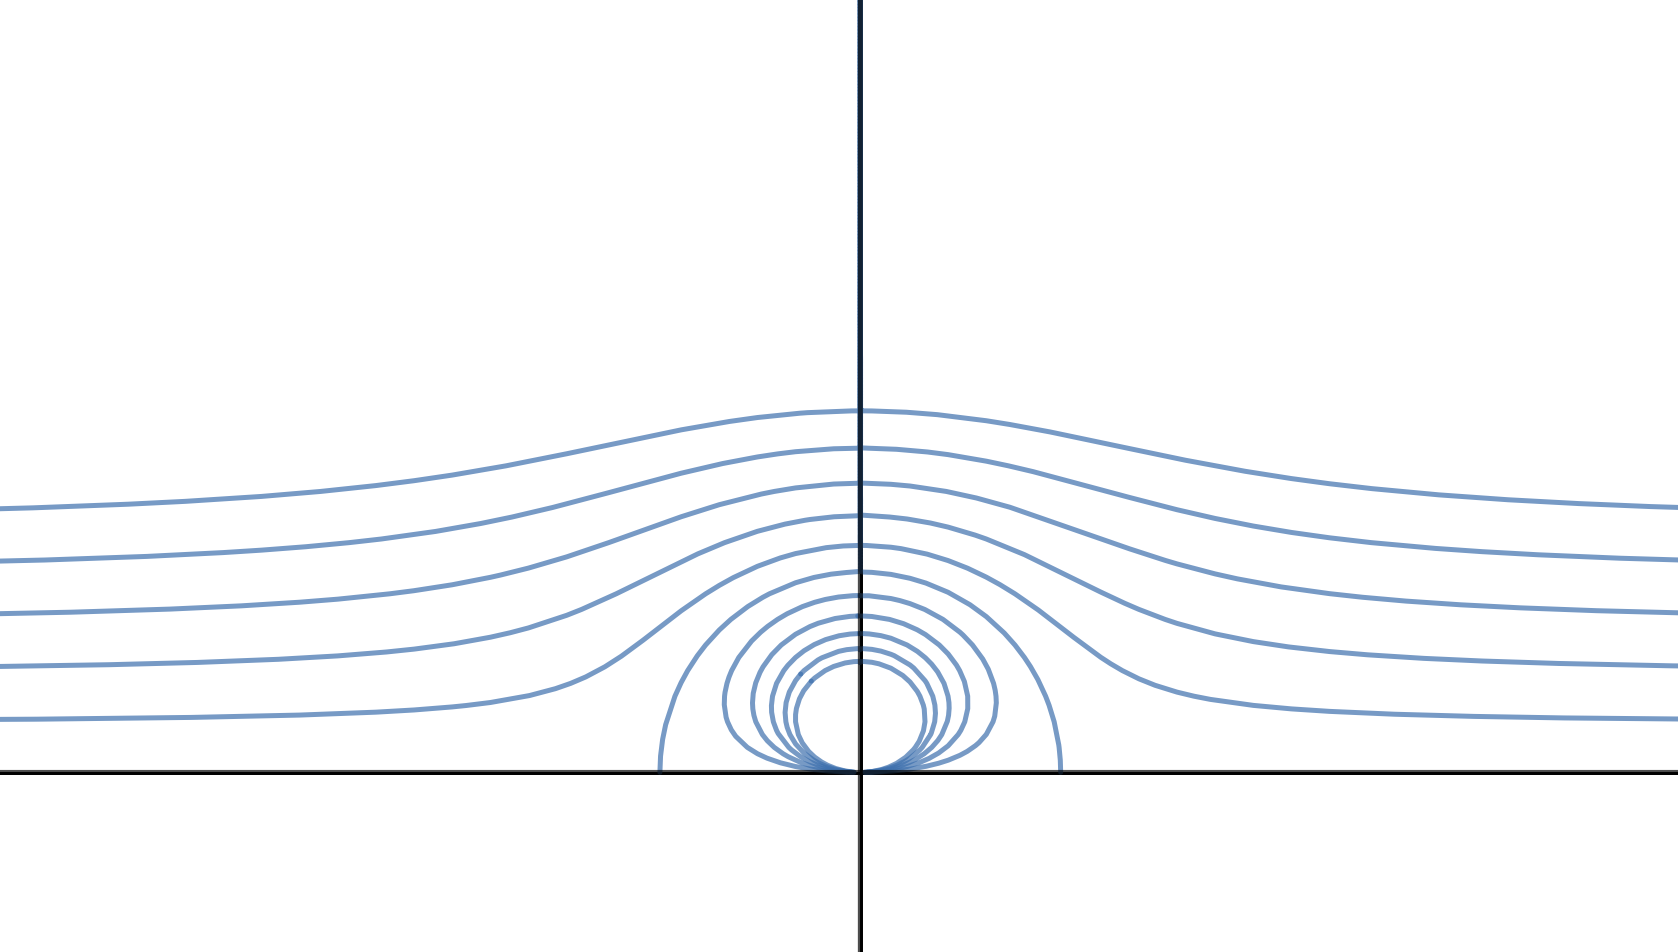
\includegraphics[width=\textwidth]{Streamlines_3.png}
			\end{center}
			\end{figure}

			\bigbreak

			\item We are now required to find the stagnation points of the fluid flow. In order to find these points, we set $\displaystyle{\frac{dw}{dz}=0}$, and solve for $\displaystyle{z}$. Thus, we compute the stagnation points using the following proof.

			\begin{align*}
			\frac{dw}{dz} & = 0\\
			U\left(1 - \frac{1}{z^2}\right) & = 0\\
			1 - \frac{1}{z^2} & = 0\\
			1 & = \frac{1}{z^2}\\
			\therefore z^2 & = 1\\
			\therefore z & = \pm 1\\
			\end{align*}

			Thus the stagnation points occur at $\displaystyle{z = 1}$ and $\displaystyle{z = -1}$.


		\end{enumerate}


	\end{enumerate}

\end{enumerate}


\end{document}
